\documentclass[11pt,a4paper]{article}
\usepackage[utf8x]{inputenc}
\usepackage[T1]{fontenc}
\usepackage[english]{babel}
\usepackage{graphicx}
%\usepackage[top=2cm, bottom=2cm, left=2cm, right=2cm]{geometry}
\usepackage[top=3cm, bottom=3cm, left=3cm, right=3cm]{geometry}
\usepackage{amsmath}
\usepackage{amsfonts}
\usepackage{amssymb}
\usepackage{pdfpages}
\usepackage{setspace}
\usepackage{hyperref}
\usepackage{tikz}

%%%%%%%%%%%%%%%%%%%%%%%%%%%%%%%%%%%%%%%%%%%%%%%%%%%%%%%%%%%%%%%%%%%%%%%%
%%
%%          Gestion des pdf
%%
%%             initialisation de hypersetup
%%                 
%%
%%%%%%%%%%%%%%%%%%%%%%%%%%%%%%%%%%%%%%%%%%%%%%%%%%%%%%%%%%%%%%%%%%%%%%%%

\hypersetup{%
backref=true,%permet d'ajouter des liens dans...
pagebackref=true,%...les bibliographies
hyperindex=true, %ajoute des liens dans les index.
colorlinks=true, %colorise les liens
breaklinks=true, %permet le retour à la ligne dans les liens trop longs
urlcolor= blue, %couleur des hyperliens
linkcolor= black, %couleur des liens internes
bookmarks=true, %créé des signets pour Acrobat
bookmarksopen=true,%
%si les signets Acrobat sont créés,
%les afficher complètement.
pdftitle={INFO-F405 - Computer Security - Project 1: Rainbow Tables}, %informations apparaissant dans
pdfauthor={Anthony Debruyn, Brian Delhaisse, Alexis Lefebvre and Aurélien Plisnier},%les informations du document
pdfsubject={Rainbow Tables}%sous Acrobat.
}%

%%%%%%%%%%%%%%%%%%%%%%%%%%%%%%%%%%%%%%%%%%%%%%%%%%%%%%%%%%%%%%%%%%%%%%%%

%\title{INFO-F405 - Computer Security\\Project 1: Rainbow Tables}
%\author{Anthony Debruyn, Brian Delhaisse, Alexis Lefebvre, and Aurélien Plisnier}

\begin{document}

\includepdf{pageGarde.pdf}

%\tableofcontents
%\newpage

\section{Introduction}
The project\footnote{All further details about the project can be found on the ``Université Virtuelle''.} for the course ``Computer Security'', for this year, consists of implementing a rainbow table.
\begin{figure}[!h]
	\center
	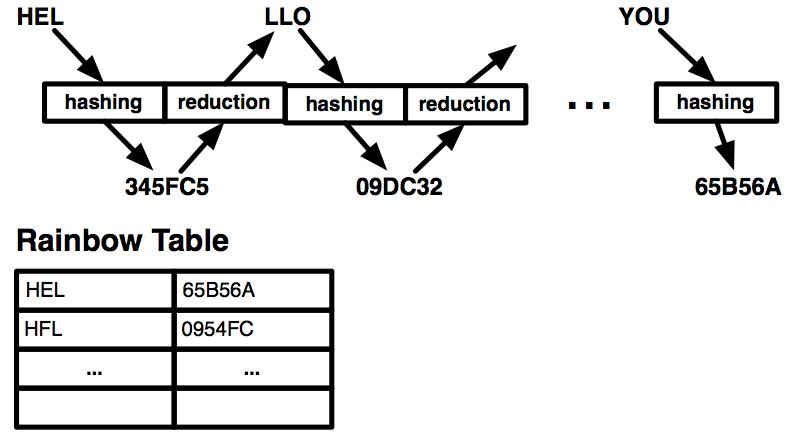
\includegraphics[scale=0.3]{HashRedRainbowTable.png}
	\caption{Sequence of reductions and hashing, and the associated rainbow table. \protect\footnotemark}
	\label{HashRedRainbowTable}
\end{figure}
This project will be implemented in C++/Java.
\footnotetext{Figure taken from the project brief made by the assistant Naïm Qachri.}

%\subsection{Algorithm to retrieve a password}
%\begin{figure}[!h]
%	\center
%	\includegraphics[scale=0.3]{Algorithm.png}
%	\caption{Algorithm to retrieve a password by using $n$ different reduction algorithms.}
%	\label{Algorithm}	
%\end{figure}
%%%%%%%%%%%% Pseudo-code : http://en.wikibooks.org/wiki/LaTeX/Algorithms %%%%%%%%%%%

\subsection{The hashing algorithm}
\begin{figure}[!h]
	\begin{center}
		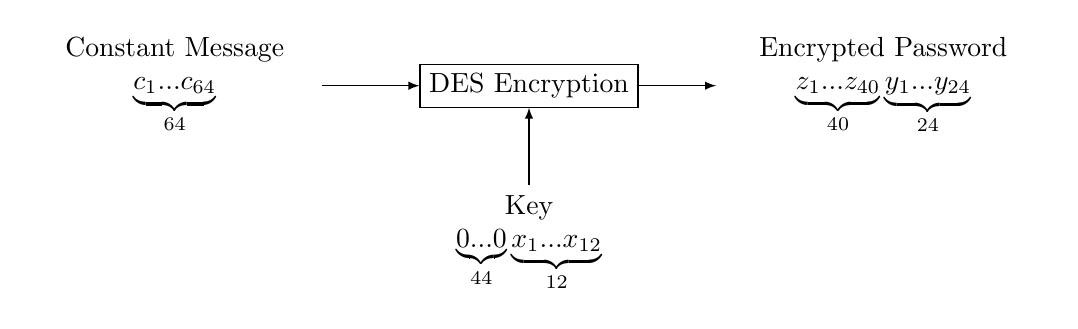
\begin{tikzpicture}[scale=1]
			\node[draw,rectangle] (DES) at (0,0) {DES Encryption};
			\node[text width=3.5cm,text centered] (Mes) at (-4.5,0) {Constant Message \\ $\underbrace{c_1...c_{64}}_{64}$};
			\node[text width=2cm,text centered] (Key) at (0,-2) {Key $\underbrace{0...0}_{44} \underbrace{x_{1}...x_{12}}_{12}$}; 
			\node[text width=4cm,text centered] (EncText) at (4.5,0) {Encrypted Password \\ $\underbrace{z_1...z_{40}}_{40} \underbrace{y_{1}...y_{24}}_{24}$};
			\draw[->,>=latex] (Mes) -- (DES);
			\draw[->,>=latex] (Key) -- (DES);
			\draw[->,>=latex] (DES) -- (EncText);
		\end{tikzpicture}	
	\end{center}
	where $\left\{ \begin{array}{l}
         x_{1}...x_{12} = \mbox{password to be hashed.}  \\
        y_{1}...y_{24} = \mbox{fingerprint (=hashed password).}
    \end{array}
\right.$
	\caption{The hashing algorithm}
	\label{Hashing}	
\end{figure}
%where $x_{1}...x_{12}$ =  password to be hashed, and $y_{1}...y_{24}$ = hashed password = fingerprint.

\subsection{The reduction function}
\begin{figure}[!h]
	\center
	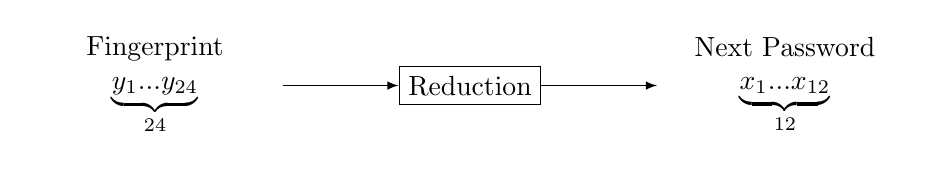
\begin{tikzpicture}[scale=1]
		%\draw (a,b) node [position] {texte}
		%\node[draw,options] (nodeName) at (x,y) {text};
		\node[draw,rectangle] (Red) at (0,0) {Reduction};
		\node[text width=3cm,text centered] (Fingerprint) at (-4,0) {Fingerprint \\ $\underbrace{y_1...y_{24}}_{24}$};
		%\node[text width=2cm,text centered] (Key) at (0,-2) {Key $\underbrace{0...0}_{44} \underbrace{x_{1}...x_{12}}_{12}$}; 
		\node[text width=3cm,text centered] (Password) at (4,0) {Next Password \\ $\underbrace{x_1...x_{12}}_{12}$};
		\draw[->,>=latex] (Fingerprint) -- (Red);
		%\draw[->,>=latex] (Key) -- (Red);
		\draw[->,>=latex] (Red) -- (Password);
		%\node[text width=3cm,text centered] (legend) at (4,0) {$x_{1}...x_{12}=$ password to be hashed};
	\end{tikzpicture}	
	\caption{The reduction function}
	\label{Reduction}	
\end{figure}

\newpage
\section{The reduction functions}
\subsection{1th reduction function}
\subsection{2nd reduction function}
\subsection{3rd reduction function}
\subsection{4th reduction function}

\newpage
\section{Description of the code}

\subsection{The class Main}

Create an item of type "CrackerRainbow" and calls its method "findPassword" in a do while loop. \\
In each turn of the loop, the user is asked to type a stolen fingerprint at each and he is given the resulting password. \\



\subsection{The class CrackerRainbow}

This is the main class of the project: it implements the algorithm given in the project assignments. \\
\item[Constructor :] Instantiates an item of class "RainbowTable" called RT.
\item[Destructor :] Deletes RT.
\item[findPassword :] The implementation of the algorithm given in the project assignments.\\ 
If the stolen fingerprint is in the rainbow table, the variable "password" is set to the corresponding password in the rainbow table. Then a method from the rainbow table is called to find the real password (branch "1" of the algorithm). \\
If the stolen fingerprint is not in the rainbow table, the variable "foundInRT" is set to false and we enter the branch "2" of the algorithm. The reduction and hashing functions are applied to the stolen fingerprint to find one stored in the rainbow table: we do it "backward" (4th reduction function then 3rd + 4th then 2nd + 3rd + 4th then 1st + 2nd + 3rd + 4th). This way, if we have as many chances to find a corresponding fingerprint during any of the 4 passes, we quicken the execution since the quickest solution is tried first. \\ If we do find a corresponding fingerprint, we jump to branch "1", if we don't the algorithm is stopped. \\

\subsection{The class RainbowTable}

\item[Constructor :] Since we use 4 reduction functions, we decided to fill the rainbow table with a quarter of the dictionary. \\ In the constructor we have a main loop going through all the passwords of the dictionary.
If the considered password is still available, we hash the password then apply the first reduction function and store the new found password then do it again so we apply all our 4 reduction functions. We then check the presence of the computed fingerprint in the rainbow table. If it is not already in the table it is stored with the corresponding password and the availabilities in the dictionary of the 4 intermediary passwords are set to false. 

\item[checkRainbowTable :] Receives a boolean and a fingerprint and applies a dichotomous search in the rainbow table. \\
If the given fingerprint in found, the boolean is set to true and we return the corresponding password. \\

\item[checkRainbowTable :] Receives a password and applies the branch "1" of the algorithm given in the project assignments to find the "real" password. \\

\item[addEntry :] Receives a password and a corresponding fingerprint. Stores the couple in the rainbow table at their right place using dichotomy. The rainbow table is ordered by fingerprints. \\

\subsection{The class RainbowTable}

A dictionary containing all the 4096 possible passwords and their availability. \\

\subsection{The library HashReduc}

This library contains our 4 reduction functions and the hashing function using DES-ECB encryption.

\newpage
\section{Conclusion}
\end{document}